\subsection{Identified particle \vn}\label{sec:identified_particle_vn}


\begin{figure}[!htb]
\begin{center}
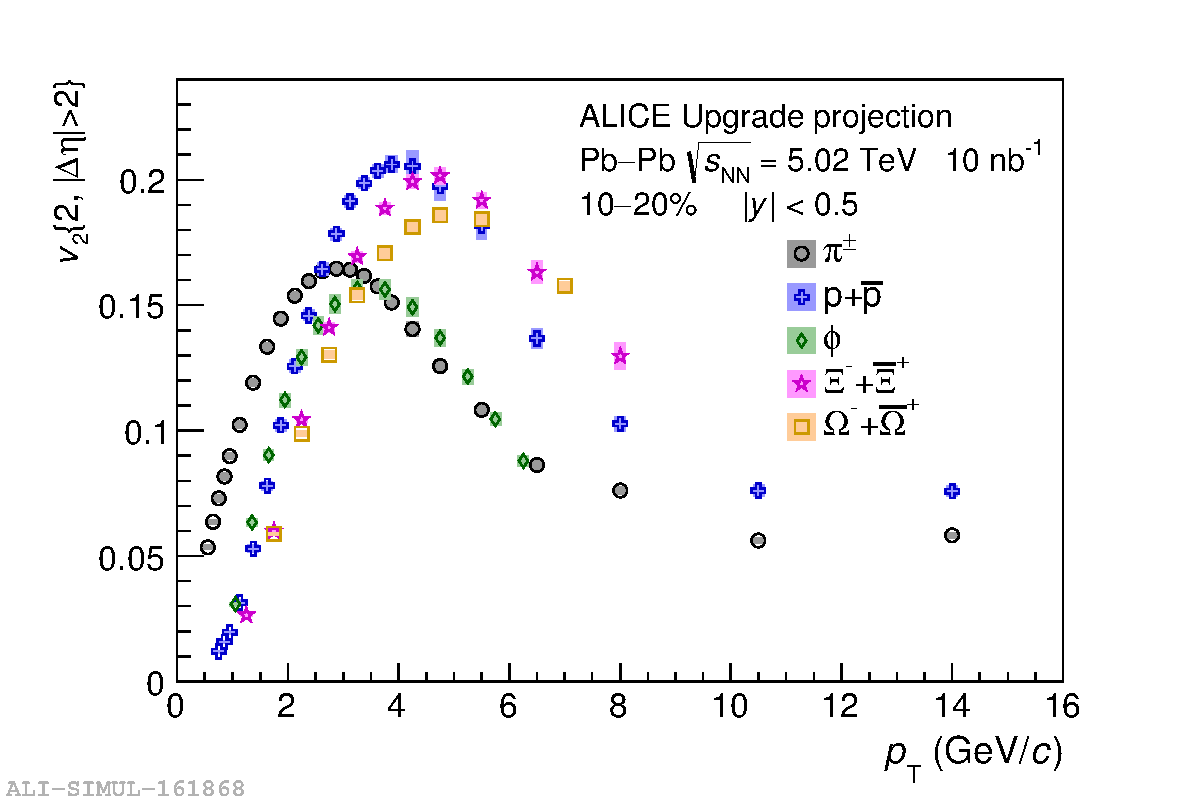
\includegraphics[width=0.495\textwidth]{\main/flow/figs/alice_projection_pid_v2}
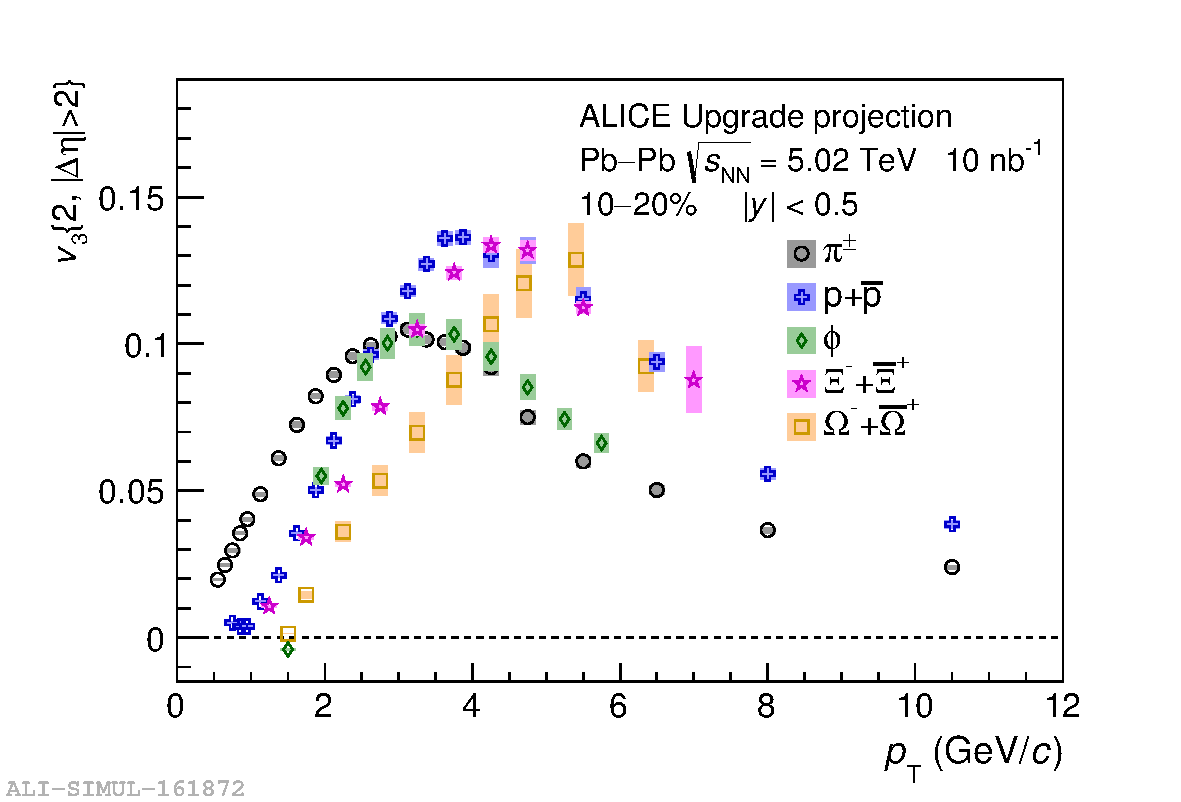
\includegraphics[width=0.495\textwidth]{\main/flow/figs/alice_projection_pid_v3}
\caption{
ALICE projections for $v_2$ (left) and $v_3$ (right) of $\pi^\pm$, 
  $\mathrm{p}$+$\overline{\mathrm{p}}$, $\Xi$+$\overline{\Xi}$, 
  $\Omega$+$\overline{\Omega}$, and the $\phi$-meson 
  in the 10--20\% centrality interval
  for an integrated luminosity of 10~nb$^{-1}$. 
Error bars (shaded boxes) represent the projected statistical 
  (systematic) uncertainties.}
\label{fig:alice_vn}
\end{center}
\end{figure}

As stated earlier most \vn\ measurements for inclusive hadrons are the LHC 
  are not statistics limited.
However for identified particles there is considerable scope for reduction 
  in statistical uncertainties in Run~3 and 4.
This is true both for heavy-flavor particles 
  as well for identified light flavour hadrons.
Figure~\ref{fig:alice_vn} shows projections from the ALICE collaboration for 
  the $v_2$ and $v_3$ of several light-flavor species, that are expected for 
  an integrated luminosity of 10~nb$^{-1}$ expected in Run~3 and 4.
The projected statistical uncertainties are typically negligible over the 
  entire \pt\ range and in most cases the systematic uncertainties are 
  quite small as well.

As stated before, the increased precision of these measurements will help in 
  better understanding of the QGP equation of state. 
These measurements will also lead to an improved understanding 
  of the hadronization mechanism at the QGP$\rightarrow$hadron transition.
Additionally, detailed measurements of constituent quark scaling (or its violation)
  can provide constraints on the contribution of the subsequent hadronic 
	rescattering, into the final azimuthal anisotropy of the final particles.
This is because the azimuthal anisotropy developed in the QGP phase 
  (as a function of transverse energy) is expected to scale with the 
	number of constituent quarks, while the anisotropy developed in the hadronic
	phase is different depending on the particle species.


\begin{figure}[!htb]
\begin{center}
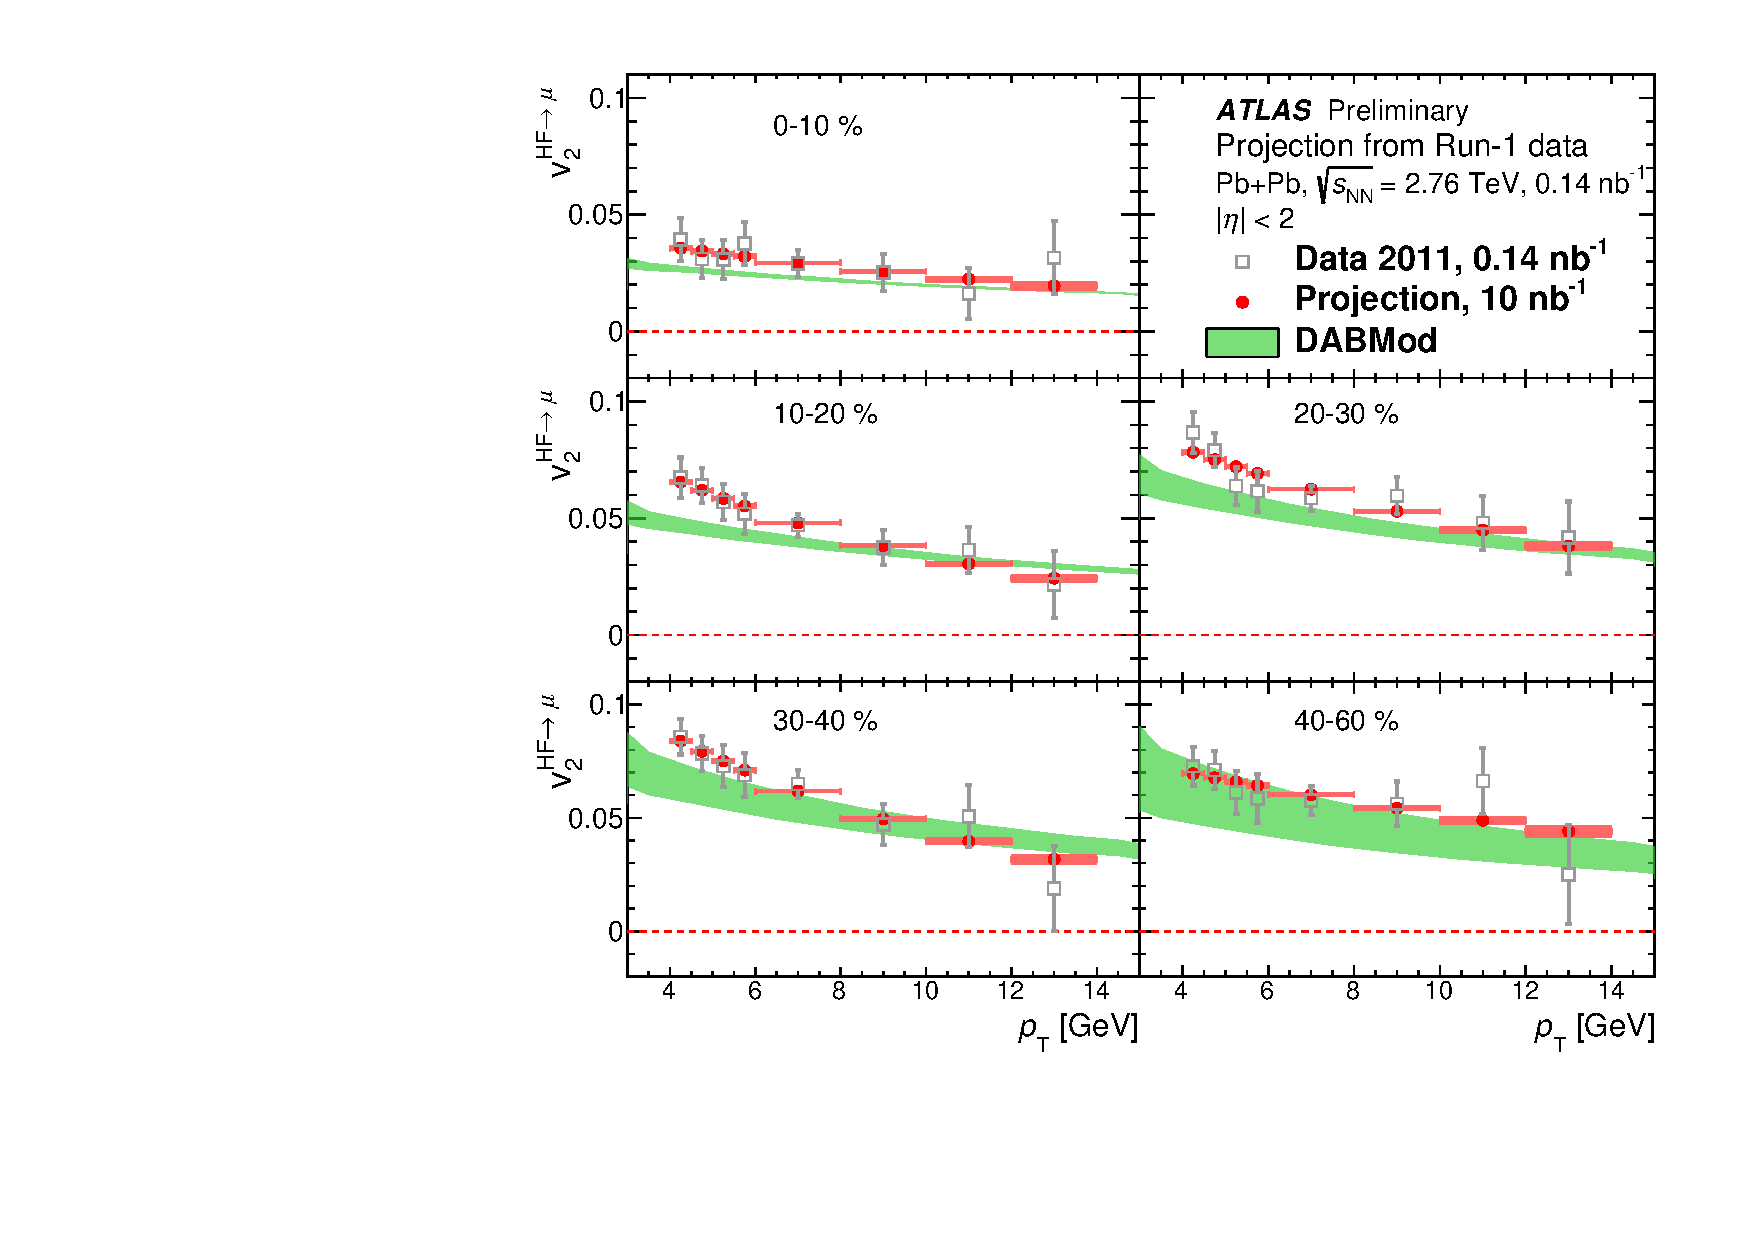
\includegraphics[width=1.0\textwidth]{\main/flow/figs/atlas_hfmuonv2}
\caption{
ATLAS projections of $v_2$ as a function of \pt, for muons from the decay of 
  heavy-flavor hadrons. 
Each panel corresponds to a different centrality interval. 
The present measurements are also shown for comparison. 
The error bars (shaded boxes) correspond to statistical uncertainties only. 
The projections are also compared to calculations from the DABMod model.}
\label{fig:atlas_hf_v2}
\end{center}
\end{figure}

Figure~\ref{fig:atlas_hf_v2} shows projections from the ATLAS collaboration
  for the $v_2$ of muons produced from the decay of heavy-flavor hadrons
  in Run~3 and 4, showing a considerable improvement in the statitical 
  precision of the measurement.
The central values of the projections are obtained by fitting the 
  present measurements with an exponential function, which qualitatively 
  describes the present data. 
The statistical uncertainties in the projections are made by scaling down 
  the present uncertainties to correspond to the expected luminosity in 
  Run~3 and 4 (10~nb$^{-1}$).
Calculations from the DABMod model~\cite{Prado:2016szr} are also shown,
  which demonstrate the inability of the present measurements
  in establishing or ruling out models due to limited statistical precision.
The flow measurements for heavy quarks is important as they are produced at
  earlier times in the heavy-ion collision and thus are susceptible
  to the full time evolution of the QGP.
The heavy-flavor anisotropy measurements can determine if heavy-quarks couple 
  strongly or weakly to the QGP, and additionally can constrain the heavy-quark 
  transport and diffusion coefficients.
Chapter~\ref{sec:HI_HF} has further discussions of Run~3 and 4 flow projections
  for heavy-flavor particles and their physics implications. 


%\subsection{QCD Equation of State}
%The QCD equation of state, accessible in high-energy collisions (and in the region around mid-rapidity) is that at vanishing baryon chemical potential, and it has been established for some time that it features a crossover transition to a chirally symmetric quark gluon plasma \cite{Aoki:2006we}. Most recent lattice calculations \cite{Steinbrecher:2018phh} have determined the cross-over temperature to be $T_c\simeq 156.5 \pm 1.5\,{\rm MeV}$. Recent efforts are also exploring the equation of state at finite $\mu_B$, which at LHC would have relevance mainly at very forward rapidities. Here, because of the sign problem, methods like Taylor expansion \cite{Kaczmarek:2011zz,Endrodi:2011gv,Bazavov:2015zja,Bonati:2018nut} or imaginary chemical potentials \cite{Cea:2014xva,Bonati:2014kpa,Bonati:2015bha,Bellwied:2015rza,Cea:2015cya} have to be employed. 

%To employ lattice QCD based equations of state in hydrodynamic caluclations, they need to be matched to a hadron resonance gas model at low temperatures, to cover the entire temperature range from zero to the maximally reached teperature. Various equations of state \cite{Huovinen:2009yb, Borsanyi:2013bia, Bazavov:2014pvz}, using different lattice data and different matching conditions have been used in simulations. A comparison of some of them can be found in \cite{Moreland:2015dvc}. In this work the sensitivity of observables to the choice of equation of state was studied. While the mean transverse momentum varied by approximately 3\% when using different equations of state, $v_2$ and $v_3$ changed by 8\% and 15\%, respectively. Because different lattice data was used, and matching to the hadron resonance gas was performed at a higher temperature, the s95p-v1 lattice parameterization has a smaller speed of sound in an extended temperature regime, compared to the other equations of state. This leads to a reduced amount of flow. 

%Such differences will affect the precise extraction of transport coefficients, such as $\eta/s$ and $\zeta/s$. Fortunately, the newer lattice QCD equations of state from the hotQCD collaboration \cite{Bazavov:2014pvz} and the Wuppertal-Budapest collaboration \cite{Borsanyi:2013bia} lead to differences only on the percent level for the studied observables.

%Currently, the experimental data can not easily teach us directly about the equation of state, because of the uncertainty in the transport coefficients. One possibility would be to extend state of the art Bayesian techniques \cite{Moreland:2018gsh} to include free parameters describing the equation of state and fit them along with other free parameters such as shear and bulk viscosities. 

%\subsection{Shear viscosity of hot nuclear matter}
%Ideal fluid dynamics has been very succesful in describing a variety of bulk observables in heavy ion collisions \cite{Kolb:2003dz,Huovinen:2003fa,Hirano:2002ds}, indicating early on that the shear and bulk viscosities of the produced matter cannot be large. Calculations in the strong coupling limit using gauge gravity duality have found a value of $\eta/s=1/4\pi$ for an $N = 4$ super Yang-Mills quantum system. This value was significantly smaller than the $\eta/s$ obtained in perturbative QCD calculations, which were, however, plagued by significant errors, mainly resulting from uncertainties in the relevant scales \cite{Arnold:2003zc}. Recently, such perturbative calculations have been extended to include next-to-leading order corrections and aa significant reduction compared to the leading order result was found \cite{Ghiglieri:2018dgf}: At temperatures of the order of the QCD transition the NLO $\eta/s$ is smaller by a factor of $5$ compared to the LO result, and reaches values of approximately $2/4\pi$. 

%Extractions of transport coefficients from lattice QCD calculations \cite{Nakamura:2004sy,Meyer:2007ic,Pasztor:2018yae} are extraordinarily hard, because the spectral function for use in the Kubo formula follows from a difficult inversion of an integral transform of a correlator of the energy momentum tensor. Most recent calcaultations for a pure gluon plasma find $\eta/s=0.17\pm 0.02$ at $T=1.5\,T_c$.

%Apart from above direct calculations of the shear viscosity to entropy density ratio, by means of hydrodynamic simulations its value can be extracted by comparison to experimental data \cite{Gale:2013da,Heinz:2013th}. This method suffers mainly from uncertainties in the initial state (see Section \ref{sec:initialstate}). The latest constraints come from simulations using the IP-Glasma initial state \cite{Schenke:2012wb,Schenke:2012fw}, the EKRT model \cite{Niemi:2015qia} and Bayesian analyses employing the Trento initial state model \cite{Moreland:2018gsh}. IP-Glasma + hydrodynamic simulations including bulk and shear viscosity find for the shear viscosity an effective constant value of $\eta/s=0.095$ at the $\sqrt{s}=2.76\,{\rm TeV}$ LHC energy and $\eta/s=0.06$ at the top RHIC energy. EKRT simulations find good agreement with LHC data using a constant value of $\eta/s=0.2$ and also certain temperature dependent $\eta/s$ values. Finally, the latest Bayesian analyses of $\sqrt{s}=5\,{\rm TeV}$ Pb+Pb collisions at the LHC using the Trento initial state determined an approximately linearly rising $\eta/s$ with temperature, with $(\eta/s)(T=150\,{\rm MeV})\approx 0.09$ and $(\eta/s)(T=300\,{\rm MeV})\approx 0.16$.

%The method of extracting $\eta/s$ using hydrodynamic simulations and comparison to experimental data thus leaves us with an uncertainty of approximately a factor of $3$ at this point. Comparison to more observables that would allow to independently better constrain features of the initial state and medium properties will hopefully reduce this uncertainty in the future. 


%\subsection{Bulk viscosity of hot nuclear matter}
%There are several theoretical indications that bulk viscosity could play an important role in the transition region of QCD (see \cite{Ryu:2017qzn} and references therein). Similar to the case of shear viscosity, bulk viscosity over entropy density ratios have been calculated using holography in the strong coupling regime using extensions to non-conformal theories \cite{Buchel:2007mf,Finazzo:2014cna}. The temperature dependent $\zeta/s$ features a peak of value 0.05 around a temperature of $\sim 160\,{\rm MeV}$. 
%Perturbative calculations have shown that the simple estimate $\zeta\approx 15 \eta(1/3-c_s^2)^2$ \cite{Horsley:1985dz} is parametrically correct for QCD \cite{Arnold:2006fz}, where $(1/3-c_s^2)$ is the deviation from conformal symmetry. Lattice calculations using the Kubo formula extract large values of $\zeta/s$ around $T_c$ \cite{Karsch:2007jc,Meyer:2007dy}, with large uncertainties for the value at $T_c$, which is of order 1 \cite{Kharzeev:2007wb}, and exhibit a fast drop with increasing $T$.

%Parametrizations of the bulk viscosity over entropy density's temperature dependence were performed in \cite{Denicol:2009am} with input from \cite{Karsch:2007jc} for the QGP phase and \cite{NoronhaHostler:2008ju} for the hadronic phase. This parametrization features a peak of $\zeta/s$ around $T\approx 180\,{\rm MeV}$, reaching approximately a value of 0.3. It has been used in various hydrodynamic simulations employing the IP-Glasma initial state and led to good agreement of the calculated mean transverse momentum with experimental data. Calculations using other initial states have reported the need for smaller bulk viscosity over entropy density values. For example in a recent Bayesian analyss using the Trento initial state model, $\zeta/s$ peaks at a value about 10 times smaller. In \cite{Schenke:2018fci} it was discussed how the compact size and initial flow present in the IP-Glasma initial state contribute to the need for a larger bulk viscosity compared to other initial state models. 

%Viscous corrections to the distribution function at freeze-out affect the low $p_T$ part of the spectrum more for bulk viscosity than for the shear part \cite{Bozek:2009dw,Paquet:2015lta}. Consequently, the uncertainties resulting from bulk viscous corrections are typically larger than for shear when studying $p_T$ integrated observables. 

%\subsection{Heat conductivity}
%Bulk diffusion, can we constrain it?

%\subsection{Electric conductivity}
%can we constrain it? Relevance for magnetic fields, Chiral magnetic effect
%
% Bulk diffusion and electric conductivity are now being discussed in the section on light flavors. (Stefan F.)
%


%\subsection{Second order transport properties}
%A peculiar feature of relativistic fluid dynamics is that it is not always causal. More specifically,  this problem arises when one goes beyond the ideal fluid approximation and includes dissipative transport properties such as shear viscosity,  bulk viscosity and heat conductivity or baryon diffusion. Keeping for the shear stress,  bulk viscous pressure and baryon diffusion current only terms of first order in gradients of the fluid velocity,  temperature and chemical potential leads to a covariant version of the well known Navier-Stokes theory,  which however,  is not an hyperbolic differential equation and can therefore not be used for a time evolution that is causal in the relativistic sense. A way out has been proposed by Müller,  as well as Israel and Stewart. In their framework,  the theoretical setup is modified in such a way that the shear stress,  bulk viscous pressure and baryon diffusion current are not related to the gradients of fluid velocity and thermodynamic variables by constraints but rather have their own evolution equation and relax towards the Navier-Stokes values on a proper time scale given by their respective relaxation times. These relaxation times cannot be too small in order to have a causal set of fluid dynamic evolution equations.

%It would in fact be great to test the modifications proposed by Müller,  Israel and Stewart (and subsequent authors) experimentally and to put an experimental bound on the value of the relaxation times (or their ratios to other thermodynamic and transport properties). This would help for a better understanding of relativistic fluid dynamics that is also needed elsewhere,  for example in cosmology. However,  this is not very easy and can only be done in an interplay of theory and experiment. In fluid dynamic models of heavy ion collisions one can vary the value of second order transport coefficients and study the impact on various flow observables,  in particular particle spectra,  flow coefficients $v_n$,  flow correlation functions and HBT parameters. By a detailed comparison to experimental data one can put constraints on the second order transport coefficients. It might become possible to vary second order transport coefficients in global Bayesian analysis calculations and provide experimental constraints in this way. A large variety of experimental flow observables,  detailed and differential data,  as well as small statistical uncertainties are obviously helpful for this endeavor.


